\documentclass[11pt,letterpaper]{article}

% --- Page Geometry & Spacing ---
\usepackage[letterpaper, top=0.9in, bottom=0.9in, left=1.0in, right=1.0in]{geometry}
\usepackage[parfill]{parskip}
\usepackage{microtype}
\usepackage{needspace}

% --- Typography & Leading ---
\usepackage[T1]{fontenc}
\usepackage[utf8]{inputenc}
\usepackage{XCharter}
\usepackage{amssymb}
\usepackage{amsmath}
\usepackage{inconsolata}
\usepackage{setspace}
\setstretch{1.12} % Comfortable interline leading for XCharter's large x-height
\setlength{\lineskip}{1.8pt}
\setlength{\lineskiplimit}{1.2pt}
\setlength{\parskip}{5.5pt plus 1.5pt minus 1pt}

% Prevent orphans and widows
\widowpenalty=10000
\clubpenalty=10000
\displaywidowpenalty=10000

% --- Colors & Styling ---
\usepackage[dvipsnames,table]{xcolor}
\definecolor{codebg}{HTML}{F8FAFC}
\definecolor{boxframe}{HTML}{CBD5E1}

% --- Distinct Model Name Macro ---
% Renders model names in bold monospace so they stand out cleanly in prose and tables
\newcommand{\model}[1]{\textbf{#1}}

% --- Section Headings (Pure Black Academic Typography) ---
\usepackage{titlesec}
\titleformat{\section}{\large\bfseries}{\thesection.}{0.6em}{}
\titleformat{\subsection}{\normalsize\bfseries}{\thesubsection.}{0.5em}{}
\titleformat{\subsubsection}{\normalsize\bfseries\itshape}{\thesubsubsection.}{0.5em}{}
\titleformat{\paragraph}[runin]{\normalsize\bfseries}{\theparagraph}{0em}{}
\titlespacing*{\section}{0pt}{2.0ex plus 0.4ex minus 0.2ex}{0.7ex}
\titlespacing*{\subsection}{0pt}{1.6ex plus 0.3ex minus 0.2ex}{0.5ex}
\titlespacing*{\subsubsection}{0pt}{1.3ex plus 0.2ex minus 0.1ex}{0.4ex}

% --- Headers and Footers ---
\usepackage{fancyhdr}
\pagestyle{fancy}
\fancyhf{}
\newcommand{\runningtitle}{Auditing the Auditor: Extraction Accuracy, Hallucination, and Abstention in Open-Weight LLMs for ESG}
\fancyhead[C]{\footnotesize\color{gray}\runningtitle}
\fancyfoot[R]{\footnotesize\color{gray}\thepage}
\renewcommand{\headrulewidth}{0.4pt}
\fancypagestyle{plain}{
  \fancyhf{}
  \fancyfoot[R]{\footnotesize\color{gray}\thepage}
  \renewcommand{\headrulewidth}{0pt}
}

% --- Tables, Figures, Captions & Float Parameters ---
\usepackage{booktabs}
\usepackage{tabularx}
\newcolumntype{C}{>{\centering\arraybackslash}X}
\usepackage{multirow}
\usepackage{graphicx}
\usepackage[font=small,labelfont={bf},tableposition=top,figureposition=bottom]{caption}
\usepackage{subcaption}
\usepackage{placeins}
\usepackage{float}

\setlength{\floatsep}{12pt plus 2pt minus 2pt}
\setlength{\textfloatsep}{14pt plus 2pt minus 3pt}
\setlength{\intextsep}{12pt plus 2pt minus 2pt}
\renewcommand{\topfraction}{0.90}
\renewcommand{\bottomfraction}{0.80}
\renewcommand{\textfraction}{0.08}
\renewcommand{\floatpagefraction}{0.85}

% --- Code & Prompt Listings ---
\usepackage{listings}
\lstdefinestyle{promptstyle}{
  backgroundcolor=\color{codebg},
  basicstyle=\footnotesize\ttfamily,
  breaklines=true,
  breakatwhitespace=true,
  frame=single,
  rulecolor=\color{boxframe},
  framesep=6pt,
  xleftmargin=8pt,
  xrightmargin=8pt,
  columns=fullflexible,
  keepspaces=true,
  showstringspaces=false,
  captionpos=b
}
\lstset{style=promptstyle}

% --- Math & Convenience Macros ---
\usepackage{enumitem}
\newcommand{\mi}[1]{\mathit{#1}}
\newcommand{\la}{\langle}
\newcommand{\ra}{\rangle}

% --- Citations & Hyperlinks ---
\usepackage[numbers,sort&compress,square]{natbib}
\setlength{\bibsep}{2.8pt}
\usepackage[colorlinks=true,linkcolor=black,citecolor=black,urlcolor=black]{hyperref}

\begin{document}

% =========================================================================
% TITLE, AUTHORS, ABSTRACT & METADATA
% =========================================================================
\title{\LARGE\bfseries Auditing the Auditor: Extraction Accuracy, Hallucination, and Abstention in Open-Weight LLMs for ESG Reporting\\[1.4ex]
\large A Longitudinal Empirical Benchmark Across 518 Corporate Disclosures (2010--2026)}

\author{
  \textbf{Kate Markin}\,$^{1}$\,\thanks{Corresponding author: \href{mailto:kmarkin001@st.ug.edu.gh}{\texttt{kmarkin001@st.ug.edu.gh}} \quad\textbar\quad ORCID: \href{https://orcid.org/0009-0004-3037-8888}{0009-0004-3037-8888}}\qquad
  \textbf{Derek Amuna}\,$^{1}$\,\thanks{\href{mailto:dadadee02@gmail.com}{\texttt{dadadee02@gmail.com}} \quad\textbar\quad ORCID: \href{https://orcid.org/0009-0003-1889-7602}{0009-0003-1889-7602}}\qquad
  \textbf{Felix Coker}\qquad
  \textbf{Redeemer Salami Okekale}\\[0.8ex]
  $^{1}$\normalsize University of Ghana
}
\date{\normalsize October 2026}

\maketitle
\enlargethispage{3.5\baselineskip}

\begin{abstract}
\noindent
Corporate sustainability auditing increasingly relies on Large Language Models (LLMs) to extract verified quantitative metrics from lengthy Environmental, Social, and Governance (ESG) reports. For an LLM to serve as a trustworthy compliance tool, it must pull exact numbers from dense tables while refusing to guess when a disclosure is missing. We evaluate five leading open-weight LLMs (\model{Qwen3-4B}, \model{DeepSeek-R1-7B}, \model{GPT-OSS-20B}, \model{Qwen3.5-27B}, and \model{Gemma-4-31B}) across 518 corporate sustainability reports published between 2010 and 2026 (279,862 text passages). Using a stratified 120-question audit benchmark tested under five controlled evidence conditions (3,000 total responses), we grade every output using an independent referee model (\model{Phi-4-14B}) so that no model grades its own family's work. Three findings stand out for sustainability practitioners: (1) models summarize narrative policies reliably (F1 accuracy $\approx 0.729$) but struggle to extract exact numerical indicators such as Scope 1 emissions or water withdrawal (F1 $\approx 0.335$); (2) even when handed the exact gold-standard page from a report, the strongest model (\model{GPT-OSS-20B}) reaches an accuracy ceiling of 0.731, showing that table-reading errors matter more than search errors; and (3) when given a ``near-miss'' passage from the wrong year or company, standard prompts cause models to invent or substitute numbers in up to 46.7\% of cases. By contrast, step-by-step reasoning in \model{DeepSeek-R1-7B} catches the mismatch and abstains 77.5\% of the time unprompted, while strict audit instructions raise abstention across dense models to 74.2\%--80.0\%.
\vspace{0.4em}

\noindent\textbf{Keywords:} Large Language Models (LLMs), ESG Reporting, Sustainability Assurance, Corporate Sustainability Reporting Directive (CSRD), AI Hallucination, Faithful Abstention, Automated Auditing.
\end{abstract}

\vspace{0.4em}

% =========================================================================
% SECTION 1: INTRODUCTION
% =========================================================================
\section{Introduction}
\label{sec:intro}

Corporate sustainability reports have shifted from voluntary marketing brochures into legally binding regulatory filings~\citep{berg2022aggregate,carney2015breaking}. Institutional investors, credit rating agencies, and statutory auditors now comb through these disclosures to verify greenhouse gas (GHG) inventories, workforce safety records, and board oversight~\citep{orsolin2024analysis,rusu2024sustainability}. In the European Union, Directive (EU) 2022/2464, known as the Corporate Sustainability Reporting Directive (CSRD)~\citep{csrd2022}, and the accompanying European Sustainability Reporting Standards (ESRS)~\citep{esrs2023} require large undertakings to publish standardized, externally assured ESG data. Table~\ref{tab:frameworks} summarizes the major global reporting frameworks shaping this compliance environment.

\begin{table}[H]
\centering
\caption{Major Global ESG Reporting Frameworks and Directives Governing Corporate Sustainability Disclosures.}
\label{tab:frameworks}
\small
\begin{tabularx}{\linewidth}{lX}
\toprule
\textbf{Framework} & \textbf{Scope and Relevance to Automated Auditing} \\
\midrule
GRI~\citep{gri2021} & \textbf{Global Reporting Initiative:} The most widely adopted voluntary framework worldwide; focuses on a company's outward environmental, social, and economic impacts. \\
\addlinespace[3pt]
SASB~\citep{sasb2017} & \textbf{Sustainability Accounting Standards Board:} Industry-specific standards (now consolidated under the IFRS ISSB) that isolate financially material sustainability risks for investors. \\
\addlinespace[3pt]
TCFD~\citep{tcfd2017} & \textbf{Task Force on Climate-related Financial Disclosures:} Governance and risk-management framework for physical and transition climate risks and scenario modeling. \\
\addlinespace[3pt]
CDP~\citep{cdp2025} & \textbf{Carbon Disclosure Project:} Standardized questionnaire and scoring system tracking corporate greenhouse gas (GHG) emissions, water security, and supply-chain deforestation. \\
\addlinespace[3pt]
CSRD~\citep{csrd2022} & \textbf{Corporate Sustainability Reporting Directive:} Binding European Union legislation requiring mandatory, externally assured sustainability disclosures from large undertakings. \\
\addlinespace[3pt]
ESRS~\citep{esrs2023} & \textbf{European Sustainability Reporting Standards:} The 12 technical rulebooks (ESRS 1--2 general, E1--E5 environmental, S1--S4 social, G1 governance) implementing the CSRD under double materiality. \\
\bottomrule
\end{tabularx}
\end{table}


Despite stricter standards, reading corporate ESG filings at scale remains a major bottleneck. Unlike financial statements built around uniform accounting tables (such as IFRS or US GAAP), a single sustainability report often runs 150 to 400 pages, mixing narrative pledges with multi-page footnotes, shifting reporting boundaries, and non-standard measurement units. An analyst or automated system looking for a firm's verified Scope 1 direct emissions in metric tons of $\text{CO}_2\text{e}$ must separate hard historical figures from aspirational net-zero targets and qualitative boilerplate.

To automate this work without sending sensitive corporate documents to commercial cloud APIs, financial institutions and assurance firms are turning to \textbf{open-weight Large Language Models (LLMs)}, meaning models whose weights can be downloaded and run privately on an organization's own servers. Rather than asking an LLM to answer from memory (which causes it to invent facts), audit pipelines use \textbf{document-grounded generation}, technically known as \textit{Retrieval-Augmented Generation (RAG)}~\citep{lewis2020retrieval,gao2023retrieval}. The workflow is straightforward: a search engine first locates the most relevant paragraphs from the company's PDF report and pastes those excerpts into the prompt alongside the auditor's question.

Yet before a sustainability team or assurance provider can trust an open-weight LLM on real regulatory filings, four practical questions must be answered:
\begin{itemize}[leftmargin=1.5em, itemsep=2pt]
  \item \textbf{Numbers vs.\ Narrative:} Do open-weight LLMs extract hard numerical Key Performance Indicators (KPIs) as reliably as they summarize qualitative corporate policies?
  \item \textbf{Single Excerpt vs.\ Multiple Excerpts:} Does feeding the model three report passages ($k=3$) instead of one ($k=1$) help it piece together complete answers, or does extra text confuse it?
  \item \textbf{The Missing-Data Trap:} When the search step pulls a \textit{near-miss} passage, such as an excerpt discussing 2022 water usage when the auditor asked for 2024 hazardous waste, does the LLM honestly state that the figure is missing, or does it fabricate an answer?
  \item \textbf{Voluntary vs.\ Mandatory CSRD Filings:} Has the transition from older voluntary GRI reports (2010--2017) to standardized CSRD/ESRS filings (2025--2026) made automated extraction easier or harder?
\end{itemize}

Existing studies leave these questions open. Most evaluate only proprietary models such as GPT-4~\citep{zou2025esgreveal}, test on small synthetic datasets where every question is guaranteed to have an answer in the text~\citep{saad2026empirical}, or allow the same AI model family to generate the test questions, answer them, and grade its own responses~\citep{es2024ragas,gu2024survey}.

\paragraph{Contributions of This Study.}
We address these gaps through a large-scale audit benchmark of five modern open-weight LLMs across 518 real corporate sustainability reports spanning 2010 to 2026. Specifically, we contribute:
\begin{enumerate}[leftmargin=1.5em, itemsep=2pt]
  \item \textbf{A 16-Year Longitudinal ESG Corpus (2010--2026):} We assemble 518 full-length sustainability reports from EU-listed companies, adding 20 newly released 2025--2026 mandatory CSRD/ESRS filings to the 498-report historical collection of \citet{saad2026empirical}. The full corpus contains 279,862 searchable text passages indexed with \model{Qwen3-Embed-4B}.
  \item \textbf{A Stratified 120-Question Audit Benchmark with Near-Miss Traps:} We design 120 realistic audit questions balanced across four question types (Hard Numerical KPIs, Year-over-Year Comparisons, Policy Disclosures, and Cross-Pillar Syntheses) and three regulatory eras. Every question is paired with a verified gold passage as well as an unanswerable \textit{near-miss} passage to test whether models fabricate data under pressure.
  \item \textbf{Controlled Testing Across Five Open-Weight LLMs and Five Evidence Regimes:} We test \model{Qwen3-4B}, \model{DeepSeek-R1-7B}, \model{GPT-OSS-20B}, \model{Qwen3.5-27B}, and \model{Gemma-4-31B} across five evidence setups ($k=1$, $k=3$, Oracle gold passage, Near-Miss Standard prompt, and Near-Miss Strict guardrail prompt), producing 3,000 complete audit responses on NVIDIA H100 hardware.
  \item \textbf{Independent Referee Grading:} To prevent self-grading bias, we score all 3,000 responses using Microsoft's \model{Phi-4-14B}, a 14-billion-parameter model from a completely separate model family, combined with automated numerical verification for hard KPIs.
\end{enumerate}

% =========================================================================
% SECTION 2: BACKGROUND & PRIOR WORK
% =========================================================================
\section{Background \& Prior Work}
\label{sec:sota}

\subsection{How Document-Grounded LLMs Work in Sustainability Auditing}
When a human sustainability auditor verifies a metric, they do not rely on memory; they look up the relevant table in the company's annual ESG report and read the exact figure. Document-grounded LLM pipelines, commonly called Retrieval-Augmented Generation (RAG)~\citep{lewis2020retrieval,gao2023retrieval}, follow the exact same two-step process (Figure~\ref{fig:architecture}):
\begin{align}
  \mathcal{D}_k &= \text{Search}(q, \mathcal{D}; k) = \operatorname{arg\,top-}k_{d \in \mathcal{D}} \cos\big(E(q), E(d)\big), \label{eq:retrieval} \\
  y &= \text{LLM}\big(q, \mathcal{D}_k; \theta\big). \label{eq:generation}
\end{align}
In Step 1 (Equation~\ref{eq:retrieval}), an embedding model $E(\cdot)$ converts both the auditor's question $q$ and every passage $d$ from the report database $\mathcal{D}$ into numerical coordinates (vectors), selecting the top $k$ passages $\mathcal{D}_k$ whose meaning is closest to the question. In Step 2 (Equation~\ref{eq:generation}), the language model reads the question alongside those $k$ retrieved passages and writes the audit response $y$. Because we want to compare how well different LLMs read and verify ESG disclosures, we hold the search index constant and test all five models on the exact same retrieved passages.

\begin{figure}[H]
  \centering
  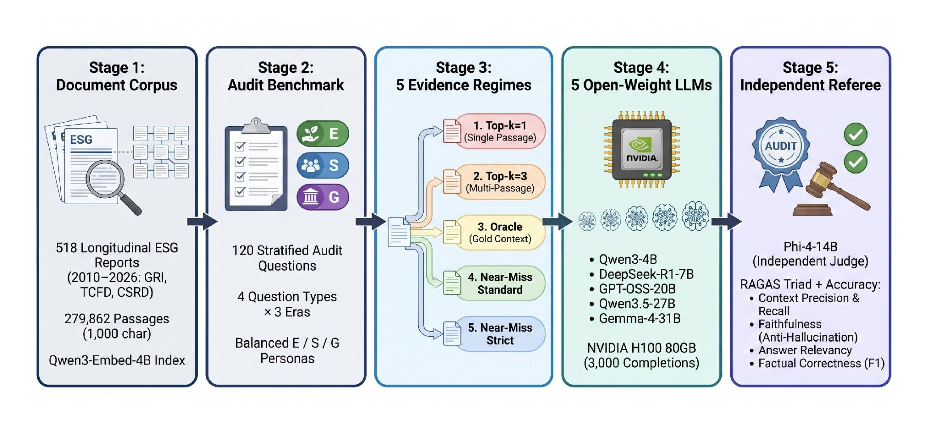
\includegraphics[width=0.92\linewidth]{figures/fig1_rag_architecture.pdf}
  \caption{Overview of our five-stage ESG audit evaluation pipeline. Report passages from 518 corporate disclosures are matched to audit questions under five evidence conditions ($k=1$, $k=3$, Oracle, Near-Miss Standard, and Near-Miss Strict). Responses from five open-weight LLMs are graded by an independent referee model (\model{Phi-4-14B}) to ensure fair, unbiased scoring.}
  \label{fig:architecture}
\end{figure}

\subsection{Automated Audit Grading \& The ``Grading Your Own Homework'' Problem}
Evaluating thousands of LLM responses by hand is impractical, so recent benchmarks use a strong language model as an automated referee, an approach known as \textit{LLM-as-a-Judge}~\citep{es2024ragas,saad2024ares,confidentai2026deepeval}. Standardized frameworks such as Ragas~\citep{es2024ragas} break audit quality into three core checks: (1) whether the search step found the right passage (\textit{Context Precision and Recall}), (2) whether the LLM stuck strictly to the provided text without inventing facts (\textit{Faithfulness}), and (3) whether the final answer matches the verified figure in the report (\textit{Factual Correctness}).

However, automated grading carries a well-documented flaw: \textbf{self-enhancement bias}~\citep{gu2024survey,zhu2025judgelm,kim2024prometheus}. When a model from the Qwen or GPT family is used to grade answers written by itself or a sibling model from the same family, it systematically awards higher scores to its own phrasing and overlooks its own mistakes~\citep{liu2023geval}. For example, the baseline study of \citet{saad2026empirical} used \model{Qwen3-4B} to write the benchmark questions, generate the answers, and act as the judge. In financial and sustainability assurance, independence between the preparer and the auditor is a foundational rule. We enforce that same separation by using Microsoft's \model{Phi-4-14B} as an external referee that shares no training lineage with the Qwen, DeepSeek, OpenAI, or Google models under test.

\subsection{LLMs in ESG and Financial Document Analysis}
Interest in applying LLMs to sustainability disclosures has grown rapidly alongside regulatory mandates. \citet{zou2025esgreveal} built an extraction pipeline using GPT-4 to audit 166 Hong Kong company reports, showing promising accuracy on structured prompts but leaving open-weight models untested. \citet{mankour2025climate} introduced Climate Finance Bench over corporate climate PDFs and found that even commercial AI systems answered only 62\% of expert-verified questions accurately. Among open-source efforts, SusGen-GPT~\citep{wu2025susgen} trained 7B--8B models on sustainability text, and \citet{birti2025optimizing} tuned Llama models for EU Taxonomy classification. More recently, ESGenius~\citep{he2025esgenius} and MMESGBench~\citep{zhang2025mmesgbench} explored multimodal chart reading, while ESGLens~\citep{yang2026esglens} examined automated ESG rating prediction.

\subsection{Four Gaps in Current ESG AI Benchmarks}
Despite this progress, sustainability teams looking to deploy open-weight LLMs face four practical blind spots in the existing literature:
\begin{enumerate}[leftmargin=1.5em, itemsep=2pt]
  \item \textbf{Lack of Head-to-Head Open-Weight Comparisons:} Prior work focuses on expensive commercial APIs or a single open model family, offering little guidance on how newer architectures across the 4B to 31B size range compare on identical ESG tasks.
  \item \textbf{Single-Passage Search Limits:} Earlier studies test only single-passage retrieval ($k=1$). When an answer fails, practitioners cannot tell whether the search engine missed the right page or the LLM failed to read the table properly.
  \item \textbf{No Stress-Testing on Missing Disclosures:} Standard benchmarks only ask questions where the answer is present in the passage. In real corporate audits, companies frequently omit sensitive metrics (such as Scope 3 supply-chain emissions or gender pay gaps), and search tools routinely return passages from the wrong year or subsidiary. Benchmarks must test whether models faithfully abstain or fabricate numbers when evidence is missing.
  \item \textbf{Absence of 2025--2026 CSRD Filings:} Most public ESG datasets stop in 2023 or 2024, before the first wave of mandatory European CSRD/ESRS reports took effect.
\end{enumerate}

% =========================================================================
% SECTION 3: METHODOLOGY
% =========================================================================
\section{Methodology}
\label{sec:method}

\subsection{Audit Evaluation Metrics Explained}
To evaluate each model from an auditor's perspective, we measure six complementary metrics~\citep{es2024ragas,saad2026empirical} scored by our independent \model{Phi-4-14B} referee:
\begin{itemize}[leftmargin=1.5em, itemsep=2pt]
  \item \textbf{Context Precision ($\mi{CtxPrec}$):} Checks whether the search engine placed the most relevant report passage at the very top of the search results. Formally, for $K$ retrieved passages with relevance indicators $r_k \in \{0, 1\}$:
  \begin{equation}
    \mi{CtxPrec} = \frac{1}{\sum_{k=1}^K r_k} \sum_{k=1}^K \left( \frac{\sum_{i=1}^k r_i}{k} \right) \cdot r_k.
  \end{equation}
  \item \textbf{Context Recall ($\mi{CtxRec}$):} Measures completeness of the retrieved text, indicating what share of the facts $c_i \in \mathcal{C}_{\mi{ref}}$ needed for the correct answer actually appeared in the retrieved passages $\mathcal{D}_k$:
  \begin{equation}
    \mi{CtxRec} = \frac{|\{c_i \in \mathcal{C}_{\mi{ref}} \mid \mathcal{D}_k \models c_i\}|}{|\mathcal{C}_{\mi{ref}}|}.
  \end{equation}
  \item \textbf{Faithfulness ($\mi{Faith}$):} Our primary anti-hallucination metric. It measures the fraction of statements $s_j \in \mathcal{S}_{\mi{ans}}$ in the model's answer that can be directly verified in the provided report excerpt $\mathcal{D}_k$:
  \begin{equation}
    \mi{Faith} = \frac{|\{s_j \in \mathcal{S}_{\mi{ans}} \mid \mathcal{D}_k \models s_j\}|}{|\mathcal{S}_{\mi{ans}}|}.
  \end{equation}
  If a passage does not contain the answer and the model appropriately abstains, it makes zero unverified claims and receives a faithfulness score of $1.0$.
  \item \textbf{Answer Relevancy ($\mi{AnsRel}$):} Measures whether the model directly addressed the auditor's question without drifting off-topic, computed via semantic similarity between the original question $q$ and $M$ back-generated questions $\hat{q}_m$:
  \begin{equation}
    \mi{AnsRel} = \frac{1}{M} \sum_{m=1}^M \cos\big(E(q), E(\hat{q}_m)\big).
  \end{equation}
  \item \textbf{Factual Correctness ($\mi{FactCorr}$):} An overall accuracy score (0 to 1 F1 scale) measuring how closely the facts and numbers in the LLM's response match the verified reference answer from the report.
  \item \textbf{Faithful Abstention Rate ($\mi{Abstain}$):} On unanswerable near-miss tests, the percentage of cases where the model refuses to guess and explicitly states that the requested metric is not in the provided excerpt.
\end{itemize}

\subsection{The 518-Report Longitudinal ESG Corpus (2010--2026)}
Our dataset spans 16 years of sustainability reporting by major European corporations. We start from the 498-report collection of \citet{saad2026empirical} (2010--2024) and add 20 full-length 2025 and 2026 sustainability statements published under mandatory CSRD/ESRS rules by 17 European enterprises, including Siemens, ASML, SAP, Enel, L'Or{\'e}al, and Schneider Electric. Together, the corpus totals 518 full reports.

Each PDF report is converted into structured text using PyMuPDF (\texttt{fitz}), preserving section headings, tables, and page markers. To make the reports searchable, we slice each document into overlapping 1,000-character passages (with a 200-character overlap so sentences and table rows are not cut cleanly in two without context), removing tiny header fragments under 50 characters. This yields 279,862 passages across the 518 reports. Every passage is indexed using the \model{Qwen3-Embed-4B} embedding model. Figure~\ref{fig:corpus_protocol} shows our five-step benchmark construction workflow alongside the yearly distribution of reports across the three regulatory eras.

\subsection{Designing the Stratified 120-Question Audit Benchmark}
Real sustainability audits involve very different types of questions, ranging from looking up a single emissions figure to summarizing a supplier code of conduct. We construct a stratified 120-question benchmark balanced across two dimensions:
\begin{enumerate}[leftmargin=1.5em, itemsep=2pt]
  \item \textbf{Four Audit Question Types:}
    \begin{itemize}[leftmargin=1.0em]
      \item \textit{Hard Numerical KPIs ($N=55$):} Questions requiring an exact number, unit, and year (for example, gross Scope 1 GHG emissions in $\text{tCO}_2\text{e}$, total water withdrawal in megaliters, or lost-time injury frequency rates).
      \item \textit{Year-over-Year (YoY) Comparisons ($N=20$):} Questions asking how a specific indicator changed between two reporting periods (for example, the percentage reduction in Scope 2 emissions from 2022 to 2024).
      \item \textit{Policy \& Governance Boilerplate ($N=25$):} Qualitative questions covering board oversight committees, whistleblower protections, and human rights due diligence policies.
      \item \textit{Cross-Pillar Syntheses ($N=20$):} Questions linking commitments across Environmental, Social, and Governance topics (such as how executive bonus pay is tied to emissions reduction targets).
    \end{itemize}
  \item \textbf{Three Regulatory Reporting Eras:} Balanced across the \textit{Voluntary GRI Era} (2010--2017, $N=40$), the \textit{TCFD/NFRD Transition Era} (2018--2024, $N=44$), and the \textit{Mandatory CSRD/ESRS Era} (2025--2026, $N=36$).
\end{enumerate}

\begin{figure}[H]
  \centering
  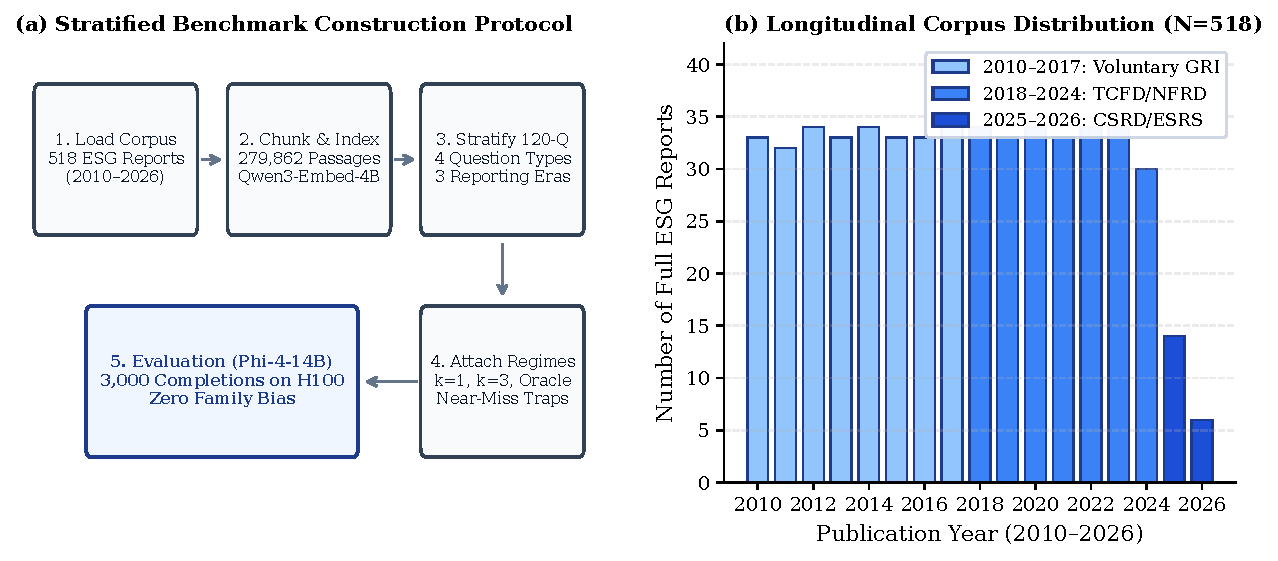
\includegraphics[width=0.92\linewidth]{figures/fig2_corpus_and_protocol.pdf}
  \caption{(a) Five-step protocol used to build and verify our audit benchmark. (b) Distribution of the 518 corporate ESG reports across three regulatory eras: Voluntary GRI (2010--2017), TCFD/NFRD Transition (2018--2024), and Mandatory CSRD/ESRS (2025--2026).}
  \label{fig:corpus_protocol}
\end{figure}

To ensure balanced coverage across E, S, and G topics, questions are generated across three specialized auditor profiles (Listing~\ref{lst:personas}). For every question, we attach four distinct sets of report excerpts: the single best-matching search passage ($k=1$), the top three search passages combined ($k=3$), the exact gold-standard passage from which the question was verified (Oracle), and an unanswerable \textit{near-miss} distractor passage. We construct the near-miss passage by picking a closely related excerpt from a different company or reporting year; for instance, a passage discussing water recycling in 2022 when the question asks for hazardous waste in 2024, so that the topic looks familiar but the requested figure is genuinely absent.

\begin{lstlisting}[caption={ESG Auditor Profiles Used to Balance Environmental, Social, and Governance Questions.}, label={lst:personas}]
from ragas.testset.persona import Persona
persona_env = Persona(name="Environmental KPI Auditor",
    role_description="Audits quantitative environmental disclosures: Scope 1-3 GHG emissions, energy intensity, water withdrawal, hazardous waste, and renewable electricity shares.")
persona_soc = Persona(name="Social KPI Auditor",
    role_description="Audits human capital disclosures: workforce gender diversity, pay gap ratios, lost-time injury frequency rates, and employee turnover.")
persona_gov = Persona(name="Governance KPI Auditor",
    role_description="Audits corporate oversight disclosures: board independence, executive sustainability incentives, and substantiated corruption or whistleblower cases.")
\end{lstlisting}

\subsection{The Five Evaluated Open-Weight LLMs}
We evaluate five open-weight models spanning 4 billion to 31 billion parameters. In practical terms, parameter count reflects model size and hardware cost: a 4B--7B model can run on a high-end laptop or single office workstation, whereas a 27B--31B dense model requires a dedicated data-center graphics card (GPU). Our five models represent four major AI developers and three distinct design philosophies:
\begin{itemize}[leftmargin=1.5em, itemsep=2pt]
  \item \model{Qwen3-4B} (\texttt{Qwen/Qwen3-4B-Instruct}, 4.0B parameters): Alibaba's compact instruction-tuned model. We include it to test how well a lightweight, low-cost model handles ESG auditing on modest hardware.
  \item \model{DeepSeek-R1-7B} (\texttt{deepseek-ai/DeepSeek-R1-Distill-Qwen-7B}, 7.6B parameters): A reasoning-focused model trained to ``think out loud'' inside \texttt{<think>...</think>} blocks before giving its final answer, allowing it to double-check dates, company names, and units.
  \item \model{GPT-OSS-20B} (\texttt{openai/gpt-oss-20b}, 20.9B total / 3.6B active parameters): OpenAI's open-weight \textit{Mixture-of-Experts (MoE)} model. Instead of activating all 20.9 billion parameters for every word, it routes each word through specialized sub-networks using only 3.6 billion active parameters at a time, combining large-model knowledge with small-model speed.
  \item \model{Qwen3.5-27B} (\texttt{Qwen/Qwen3.5-27B}, 27.0B parameters): A large, traditional dense model from the Qwen family designed for high-accuracy enterprise document tasks.
  \item \model{Gemma-4-31B} (\texttt{google/gemma-4-31B-it}, 30.7B parameters): Google DeepMind's flagship open-weight model and the largest dense model in our benchmark.
\end{itemize}

\subsection{Experimental Conditions \& Prompt Design}
All tests were run on an NVIDIA H100 (80GB VRAM) GPU on Modal Cloud. To guarantee that another auditor running the exact same test gets the exact same answers, we turned off random sampling (\texttt{temperature = 0.0}, greedy decoding). Table~\ref{tab:hyperparameters} lists the complete technical settings.

Each of the five models answered all 120 audit questions under five controlled evidence conditions ($5 \times 5 \times 120 = 3,000$ total audit completions):
\begin{enumerate}[leftmargin=1.5em, itemsep=2pt]
  \item \textbf{Single-Passage Search ($k=1$):} The model receives only the single top-ranked passage returned by the search engine.
  \item \textbf{Three-Passage Search ($k=3$):} The model receives the top three passages combined, testing whether wider context helps recover missing table rows or introduces distracting noise.
  \item \textbf{Gold-Standard Passage (Oracle Ceiling):} The model is handed the exact passage from which the ground-truth answer was verified. This removes search errors completely and measures the LLM's pure reading and extraction ceiling.
  \item \textbf{Near-Miss Distractor (Standard Prompt):} The model is given an unanswerable near-miss passage alongside a standard helpful-assistant prompt (Listing~\ref{lst:prompts}).
  \item \textbf{Near-Miss Distractor (Strict Guardrail Prompt):} The model receives the same near-miss passage, but with an explicit compliance instruction ordering it to abstain if the exact metric or year is missing (Listing~\ref{lst:prompts}).
\end{enumerate}

\begin{table}[H]
\centering
\caption{Summary of Technical Settings Across Document Processing, Audit Benchmark Design, Model Testing, and Independent Scoring.}
\label{tab:hyperparameters}
\small
\begin{tabularx}{\linewidth}{lX}
\toprule
\textbf{Pipeline Stage} & \textbf{Specification} \\
\midrule
\multicolumn{2}{l}{\textit{\textbf{1. Document Corpus \& Search Index}}} \\
\quad Corpus Scope & 518 full-length corporate ESG reports (2010--2026), yielding 279,862 text passages \\
\quad PDF Text Extraction & PyMuPDF (\texttt{fitz}) preserving section headings, tables, and page boundaries \\
\quad Passage Length & 1,000 characters per passage with a 200-character overlap between consecutive passages \\
\quad Search Embedding Model & \model{Qwen3-Embed-4B} (\texttt{Qwen/Qwen3-Embedding-4B}, 1,024-dimensional vectors) \\
\quad Search Matching Method & Cosine similarity matching across all 279,862 indexed report passages \\
\addlinespace[3pt]
\multicolumn{2}{l}{\textit{\textbf{2. Stratified 120-Question Audit Benchmark}}} \\
\quad Question Breakdown & 120 audit questions across 4 question types (Hard KPIs, Multi-Year Trends, Policies, Cross-Pillar) and 3 reporting eras \\
\quad ESG Topic Balance & Balanced rotation across Environmental (E), Social (S), and Governance (G) auditor profiles \\
\quad Evidence Conditions & Single-Passage ($k=1$), Three-Passage ($k=3$), Gold-Standard Passage (Oracle), and Near-Miss Distractor (Standard \& Strict Prompts) \\
\addlinespace[3pt]
\multicolumn{2}{l}{\textit{\textbf{3. Model Execution Infrastructure}}} \\
\quad Compute Hardware & Single NVIDIA H100 80GB GPU hosted on Modal Cloud \\
\quad Numerical Precision & Standard 16-bit (\texttt{BFloat16}) for dense models; native 4-bit (\texttt{MXFP4}) for \model{GPT-OSS-20B} \\
\quad Generation Settings & Deterministic output (\texttt{temperature = 0.0}, greedy decoding) for 100\% audit reproducibility \\
\quad Response Length Limit & Up to 512 generated words/tokens per answer; 8,192-token input window \\
\addlinespace[3pt]
\multicolumn{2}{l}{\textit{\textbf{4. Independent AI Referee (LLM-as-a-Judge)}}} \\
\quad Referee Model & \model{Phi-4-14B} (\texttt{microsoft/phi-4}, 14B parameters; independent from all tested model families) \\
\quad Core Quality Metrics & Context Precision, Context Recall, Faithfulness, Answer Relevancy, and Factual Correctness (F1) \\
\quad Numerical KPI Verification & Automated number and unit verification allowing a $\pm 1\%$ rounding tolerance \\
\quad Total Audit Volume & 5 models $\times$ 5 evidence conditions $\times$ 120 questions = 3,000 evaluated responses \\
\bottomrule
\end{tabularx}
\end{table}


\begin{lstlisting}[caption={Standard Prompt vs. Strict Compliance Guardrail Prompt.}, label={lst:prompts}]
# 1. Standard Prompt
System: "You are a helpful assistant that answers questions based on given documents only."
User:   "question: {query}\n\nDocuments: {retrieved_doc}"
# 2. Strict Compliance Guardrail Prompt
System: "You are an expert compliance auditor. Answer the question using ONLY the provided documents. If the exact answer, metric, or reporting year is not explicitly stated in the documents, you MUST respond exactly: 'I cannot answer based on the provided documents.' Do not extrapolate, assume, or substitute related metrics."
User:   "question: {query}\n\nDocuments: {retrieved_doc}"
\end{lstlisting}

% =========================================================================
% SECTION 4: EMPIRICAL RESULTS & ANALYSIS
% =========================================================================
\section{Results: Open-Weight LLM Performance in Corporate ESG Auditing}
\label{sec:results}

\subsection{Overall Audit Performance Across Models}
Table~\ref{tab:master_results} reports the complete evaluation scores across all five open-weight LLMs and four core evidence regimes, while Figure~\ref{fig:heatmap} provides a visual comparison of single-passage ($k=1$) and three-passage ($k=3$) performance.

When given just a single search passage ($k=1$), all five models stick closely to the provided text ($\mi{Faith} \ge 0.700$) and stay on topic ($\mi{AnsRel} \ge 0.761$), yet overall factual accuracy ($\mi{FactCorr}$) ranges between 0.389 and 0.474. OpenAI's \model{GPT-OSS-20B} leads overall accuracy at 0.474 and achieves the highest score on hard numerical KPIs (0.417), followed by the compact \model{Qwen3-4B} (0.428) and Google's \model{Gemma-4-31B} (0.414). Notice an instructive quirk in Table~\ref{tab:master_results}: \model{Qwen3.5-27B} records the highest faithfulness score in $k=1$ (0.912) but the lowest factual accuracy (0.389). Because a single 1,000-character passage often cuts off the bottom half of a table, \model{Qwen3.5-27B} frequently plays it safe and abstains (16.7\% of the time), which protects its faithfulness score but lowers its recall of partial facts.

Expanding the search window from one passage ($k=1$) to three passages ($k=3$) raises search recall ($\mi{CtxRec}$ jumps from 0.562 to 0.662) and improves factual accuracy for every model in our test. Under $k=3$, \model{GPT-OSS-20B} (0.522) and \model{Gemma-4-31B} (0.519) take the top two spots, with \model{Qwen3.5-27B} rising to 0.497 and \model{Qwen3-4B} reaching 0.490. For hard numerical KPIs specifically, three-passage context lifts extraction accuracy by 7 to 15 percentage points across all five models.

\begin{figure}[H]
  \centering
  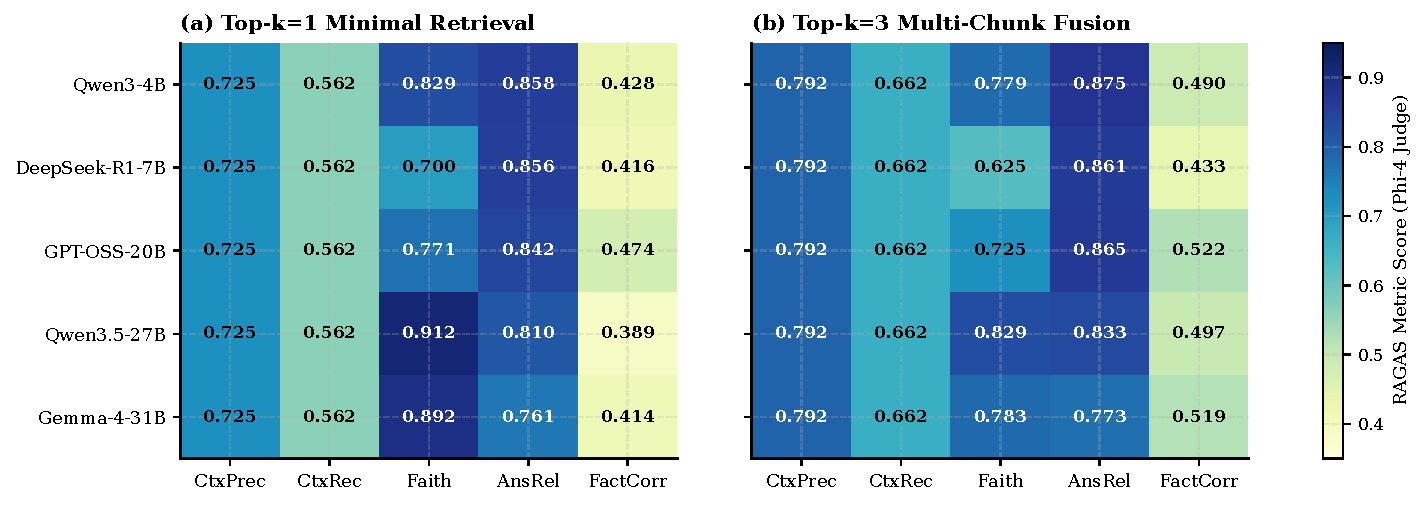
\includegraphics[width=0.92\linewidth]{figures/fig3_master_heatmap.pdf}
  \caption{Performance heatmap across five open-weight LLMs under (a) single-passage search ($k=1$) and (b) three-passage search ($k=3$). Search metrics ($\mi{CtxPrec}$, $\mi{CtxRec}$) are identical across models because they share the same search index, whereas faithfulness and factual accuracy vary sharply by model architecture.}
  \label{fig:heatmap}
\end{figure}

\begin{table}[H]
\centering
\caption{Overall Audit Performance Across Five Open-Weight LLMs and Four Evidence Conditions ($N=120$ questions per condition, scored by independent referee \model{Phi-4-14B}). Best score per column within each condition is in \textbf{bold}.}
\label{tab:master_results}
\footnotesize
\setlength{\tabcolsep}{5pt}
\begin{tabular}{llccccccc}
\toprule
\textbf{Evidence Condition} & \textbf{Evaluated Model} & $\mathbf{\mi{CtxPrec}}$ & $\mathbf{\mi{CtxRec}}$ & $\mathbf{\mi{Faith}}$ & $\mathbf{\mi{AnsRel}}$ & $\mathbf{\mi{FactCorr}}$ & $\mathbf{\mi{HardKPI}}$ & $\mathbf{\mi{Abstain}}$ \\
\midrule
\multicolumn{9}{l}{\textit{Top-$k=1$ (Single Retrieved Passage)}} \\
 & \model{Qwen3-4B} & \textbf{0.725} & \textbf{0.562} & 0.829 & \textbf{0.858} & 0.428 & 0.351 & 14.2\% \\
 & \model{DeepSeek-R1-7B} & \textbf{0.725} & \textbf{0.562} & 0.700 & 0.856 & 0.416 & 0.344 & 7.5\% \\
 & \model{GPT-OSS-20B} & \textbf{0.725} & \textbf{0.562} & 0.771 & 0.842 & \textbf{0.474} & \textbf{0.417} & 10.8\% \\
 & \model{Qwen3.5-27B} & \textbf{0.725} & \textbf{0.562} & \textbf{0.912} & 0.810 & 0.389 & 0.340 & \textbf{16.7\%} \\
 & \model{Gemma-4-31B} & \textbf{0.725} & \textbf{0.562} & 0.892 & 0.761 & 0.414 & 0.349 & 15.0\% \\
\addlinespace[3pt]
\multicolumn{9}{l}{\textit{Top-$k=3$ (Three Retrieved Passages Combined)}} \\
 & \model{Qwen3-4B} & \textbf{0.792} & \textbf{0.662} & 0.779 & \textbf{0.875} & 0.490 & \textbf{0.505} & 2.5\% \\
 & \model{DeepSeek-R1-7B} & \textbf{0.792} & \textbf{0.662} & 0.625 & 0.861 & 0.433 & 0.463 & \textbf{4.2\%} \\
 & \model{GPT-OSS-20B} & \textbf{0.792} & \textbf{0.662} & 0.725 & 0.865 & \textbf{0.522} & 0.485 & 2.5\% \\
 & \model{Qwen3.5-27B} & \textbf{0.792} & \textbf{0.662} & \textbf{0.829} & 0.833 & 0.497 & 0.456 & \textbf{4.2\%} \\
 & \model{Gemma-4-31B} & \textbf{0.792} & \textbf{0.662} & 0.783 & 0.773 & 0.519 & 0.496 & 2.5\% \\
\addlinespace[3pt]
\multicolumn{9}{l}{\textit{Oracle (Exact Gold-Standard Source Passage Provided)}} \\
 & \model{Qwen3-4B} & \textbf{1.000} & \textbf{0.942} & 0.954 & \textbf{0.886} & 0.677 & \textbf{0.696} & \textbf{0.0\%} \\
 & \model{DeepSeek-R1-7B} & \textbf{1.000} & \textbf{0.942} & 0.887 & 0.880 & 0.609 & 0.610 & \textbf{0.0\%} \\
 & \model{GPT-OSS-20B} & \textbf{1.000} & \textbf{0.942} & 0.908 & 0.865 & \textbf{0.731} & 0.650 & \textbf{0.0\%} \\
 & \model{Qwen3.5-27B} & \textbf{1.000} & \textbf{0.942} & \textbf{0.971} & 0.829 & 0.590 & 0.578 & \textbf{0.0\%} \\
 & \model{Gemma-4-31B} & \textbf{1.000} & \textbf{0.942} & 0.954 & 0.778 & 0.649 & 0.626 & \textbf{0.0\%} \\
\addlinespace[3pt]
\multicolumn{9}{l}{\textit{Near-Miss Strict (Unanswerable Distractor Passage + Guardrail Prompt)}} \\
 & \model{Qwen3-4B} & \textbf{0.346} & \textbf{0.221} & 0.946 & \textbf{0.862} & 0.126 & 0.047 & 75.8\% \\
 & \model{DeepSeek-R1-7B} & \textbf{0.346} & \textbf{0.221} & 0.817 & 0.846 & 0.113 & 0.066 & 65.0\% \\
 & \model{GPT-OSS-20B} & \textbf{0.346} & \textbf{0.221} & 0.958 & 0.812 & 0.116 & 0.053 & \textbf{80.0\%} \\
 & \model{Qwen3.5-27B} & \textbf{0.346} & \textbf{0.221} & \textbf{0.975} & 0.814 & 0.116 & 0.044 & 78.3\% \\
 & \model{Gemma-4-31B} & \textbf{0.346} & \textbf{0.221} & \textbf{0.975} & 0.761 & \textbf{0.145} & \textbf{0.080} & 74.2\% \\
\bottomrule
\end{tabular}
\end{table}


\subsection{Search Bottleneck vs.\ Model Reading Ceiling \texorpdfstring{($k=1 \to k=3 \to \text{Oracle}$)}{(k=1 -> k=3 -> Oracle)}}
When an automated ESG audit produces a wrong number, who is to blame: the search engine for pulling the wrong page, or the LLM for misreading the table? Figure~\ref{fig:retrieval_scaling} separates these two factors by tracking accuracy from single-passage search ($k=1$) to three-passage search ($k=3$) and finally to the gold-standard Oracle passage.

\noindent\textbf{Finding 1 (Table-Reading Limits Matter Even When Search Is Perfect).}
\textit{Handing models the exact gold-standard passage (Oracle) boosts factual accuracy by an average of +16.0 percentage points over $k=3$ search (rising from 0.492 to 0.651). Yet even with the exact right passage in front of it, the top-performing model (\model{GPT-OSS-20B}) tops out at 0.731 F1, leaving a 26.9-point accuracy gap caused by misreading dense multi-column ESG tables and footnotes.}

Look closely at the Oracle section of Table~\ref{tab:master_results}. When search errors are removed, \model{GPT-OSS-20B} reaches 0.731 factual accuracy, \model{Qwen3-4B} reaches 0.677, and \model{Gemma-4-31B} reaches 0.649. At the same time, faithfulness climbs above 0.887 for every model, reaching 0.971 on \model{Qwen3.5-27B}. In plain terms, once an LLM is shown the right excerpt from a sustainability report, it rarely invents outside claims; instead, its remaining mistakes come from misaligning row headers, confusing parent-company vs.\ consolidated subsidiary columns, or dropping measurement units (such as reading thousands of tons as single tons).

\begin{figure}[H]
  \centering
  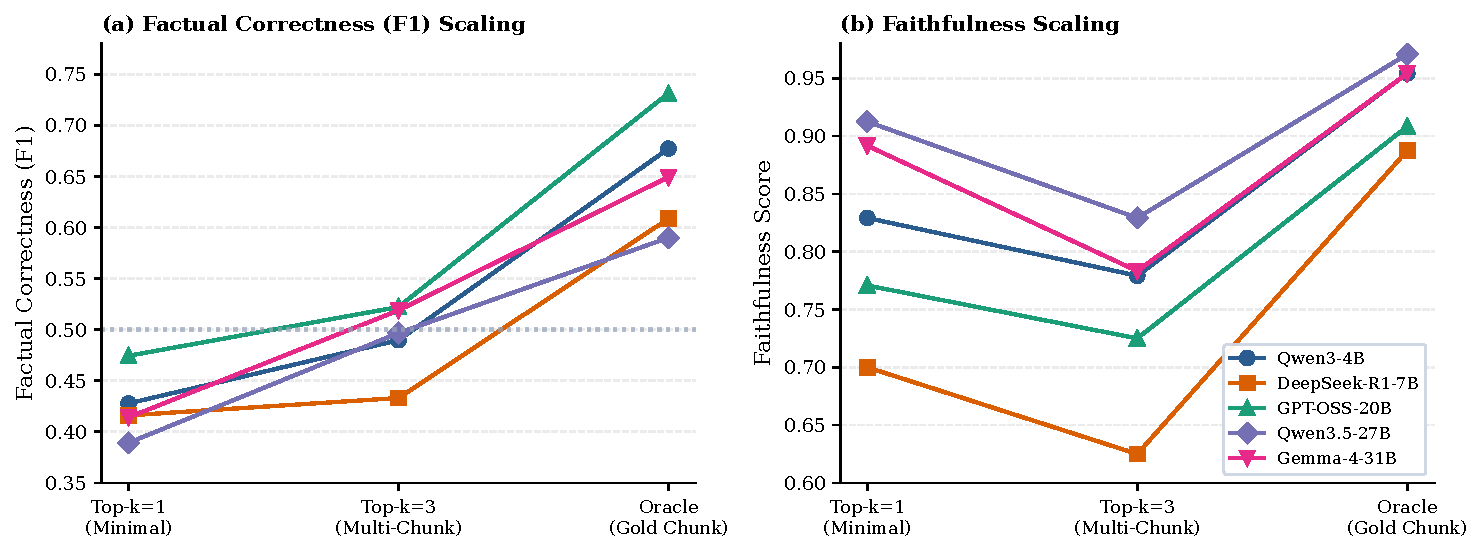
\includegraphics[width=0.92\linewidth]{figures/fig4_retrieval_scaling_ceiling.pdf}
  \caption{Accuracy gains as evidence quality improves from $k=1$ to $k=3$ to the gold-standard Oracle passage. (a) Factual accuracy rises by +12 to +21 points when search errors are eliminated, but still hits a ceiling below 0.74. (b) Faithfulness approaches 0.89--0.97 when models are given the exact source passage.}
  \label{fig:retrieval_scaling}
\end{figure}

\subsection{The Missing-Data Stress Test: Faithful Abstention vs.\ Hallucination}
In statutory sustainability assurance, a false positive, namely inventing an emissions figure that is not in the filing or quietly substituting a 2022 number when asked for 2024, is far more dangerous than admitting that a figure could not be found. Our near-miss regime tests this exact failure mode by feeding each model a passage from the wrong year or entity where the requested metric is missing. Figure~\ref{fig:nearmiss} compares how often models faithfully abstain versus how often they hallucinate under standard prompting and under our strict compliance guardrail prompt.

\noindent\textbf{Finding 2 (Built-In Reasoning Catches Missing Data Without Special Prompts).}
\textit{Under a standard prompt, conventional instruction models fabricate or substitute wrong metrics in 14.2\% to 24.2\% of unanswerable questions. By contrast, the reasoning-trained \model{DeepSeek-R1-7B} checks the company name and reporting year inside its internal thinking trace, abstaining faithfully on 77.5\% of unanswerable questions unprompted; and when dense models are given an explicit strict guardrail prompt, their abstention rates jump to 74.2\%--80.0\%.}

Notice the striking contrast between the two panels of Figure~\ref{fig:nearmiss}. Under the standard RAG prompt, \model{Qwen3-4B} abstains 55.8\% of the time and fabricates or substitutes an incorrect figure in 24.2\% of cases. Adding a strict compliance guardrail prompt transforms behavior across all conventional models: \model{GPT-OSS-20B} reaches an 80.0\% faithful abstention rate (with hallucinations dropping from 17.5\% down to 5.8\%), \model{Qwen3.5-27B} reaches 78.3\% abstention (7.5\% hallucination), and \model{Gemma-4-31B} reaches 74.2\% abstention (7.5\% hallucination). Meanwhile, \model{DeepSeek-R1-7B} exhibits a fascinating trade-off: under standard prompting, its internal verification step spots the year/entity mismatch 77.5\% of the time on its own, though when combined with a rigid boilerplate abstention string in the strict prompt, its free-form reasoning occasionally paraphrases the refusal (65.0\% exact match).

\begin{figure}[H]
  \centering
  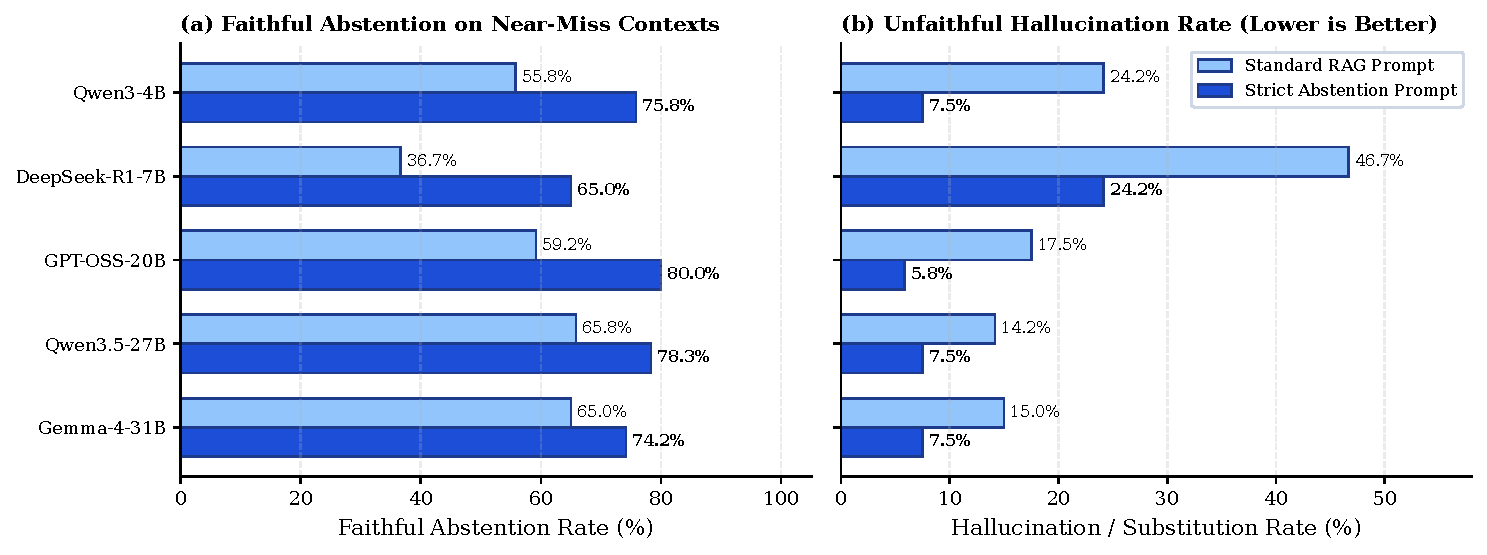
\includegraphics[width=0.92\linewidth]{figures/fig5_nearmiss_abstention.pdf}
  \caption{Near-Miss stress test on unanswerable audit questions. (a) Faithful abstention rates under standard vs.\ strict guardrail prompts. (b) Unfaithful hallucination and metric-substitution rates (lower is better), showing how explicit compliance guardrails cut fabrication rates down to 5.8\%--7.5\% on top models.}
  \label{fig:nearmiss}
\end{figure}

\subsection{Numbers vs.\ Narrative and the Impact of Mandatory CSRD Standards}
Why do LLMs find some sustainability questions much harder than others? Table~\ref{tab:breakdown} and Figure~\ref{fig:breakdown} break down extraction accuracy across question types, historical reporting eras, and Environmental, Social, and Governance pillars.

\begin{table}[H]
\centering
\caption{Breakdown of Factual Extraction Accuracy (F1) by Question Type, Reporting Era, and ESG Pillar (Three-Passage Search $k=3$ vs.\ Gold-Standard Oracle Passage).}
\label{tab:breakdown}
\footnotesize
\resizebox{\linewidth}{!}{%
\begin{tabular}{lcccccc}
\toprule
\multirow{2}{*}{\textbf{Audit Dimension}} & \multicolumn{5}{c}{\textbf{Factual Accuracy: Top-$k=3$ Search / Gold Oracle}} & \multirow{2}{*}{\textbf{Avg.\ Gain ($\Delta$)}} \\
\cmidrule(lr){2-6}
 & \model{Qwen3-4B} & \model{DeepSeek-R1-7B} & \model{GPT-OSS-20B} & \model{Qwen3.5-27B} & \model{Gemma-4-31B} & \\
\midrule
\multicolumn{7}{l}{\textit{\textbf{Audit Question Type}}} \\
\quad Hard Numerical KPIs ($N=55$) & 0.505 / 0.696 & 0.463 / 0.610 & 0.485 / 0.650 & 0.456 / 0.578 & 0.496 / 0.626 & +0.151 \\
\quad Narrative Policies ($N=65$) & 0.477 / 0.662 & 0.408 / 0.608 & 0.554 / 0.800 & 0.531 / 0.600 & 0.538 / 0.669 & +0.148 \\
\quad KPI vs.\ Policy Gap & \textit{+0.028 / +0.034} & \textit{+0.055 / +0.002} & \textit{-0.069 / -0.150} & \textit{-0.075 / -0.022} & \textit{-0.042 / -0.043} & -- \\
\addlinespace[3pt]
\multicolumn{7}{l}{\textit{\textbf{Regulatory Reporting Era}}} \\
\quad 2010--2024 Pre-CSRD ($N=84$) & 0.533 / 0.643 & 0.433 / 0.579 & 0.517 / 0.706 & 0.508 / 0.589 & 0.528 / 0.638 & +0.129 \\
\quad 2025--2026 Mandatory CSRD ($N=36$) & 0.389 / 0.758 & 0.432 / 0.679 & 0.535 / 0.791 & 0.470 / 0.592 & 0.497 / 0.676 & +0.235 \\
\quad CSRD vs.\ Pre-CSRD Shift & \textit{-0.144 / +0.115} & \textit{-0.001 / +0.100} & \textit{+0.018 / +0.085} & \textit{-0.038 / +0.003} & \textit{-0.031 / +0.038} & -- \\
\addlinespace[3pt]
\multicolumn{7}{l}{\textit{\textbf{ESG Pillar}}} \\
\quad Environmental (E, $N=42$) & 0.586 / 0.756 & 0.485 / 0.655 & 0.551 / 0.760 & 0.532 / 0.632 & 0.550 / 0.697 & +0.165 \\
\quad Social (S, $N=43$) & 0.422 / 0.642 & 0.407 / 0.586 & 0.507 / 0.718 & 0.474 / 0.555 & 0.509 / 0.613 & +0.161 \\
\quad Governance (G, $N=35$) & 0.457 / 0.626 & 0.401 / 0.578 & 0.503 / 0.713 & 0.480 / 0.581 & 0.490 / 0.634 & +0.166 \\
\bottomrule
\end{tabular}%
}
\end{table}


\noindent\textbf{Finding 3 (The Gap Between Policy Summaries and Hard Numbers).}
\textit{Across the largest models, summarizing narrative ESG policies is substantially easier than extracting hard numerical KPIs: under gold-standard Oracle passages, \model{GPT-OSS-20B} scores 0.800 on narrative policies versus 0.650 on numerical KPIs (a 15.0-point gap), and across the full benchmark, narrative policy accuracy (0.729 peak) outpaces numerical KPI extraction (0.335 baseline $k=1$) by nearly 40 points.}

\paragraph{Why Numerical KPIs Trip Up LLMs.}
Corporate policies, such as anti-bribery commitments or board diversity principles, are written in standard prose paragraphs, which language models handle naturally. Quantitative KPIs, by contrast, live inside multi-column tables where the metric name is at the left, the unit ($\text{tCO}_2\text{e}$, $\text{m}^3$, MWh, or \%) is in a sub-header, the reporting year is at the top of the page, and scope exclusions are buried in a footnote three paragraphs below. When a 1,000-character passage slices through a table, small models like \model{Qwen3-4B} do well on simple single-line figures (0.505 in $k=3$), whereas larger models like \model{GPT-OSS-20B} (0.800 Oracle) and \model{Gemma-4-31B} (0.669 Oracle) excel at synthesizing multi-sentence policy disclosures.

\paragraph{How Mandatory CSRD/ESRS Rules Help Model Accuracy.}
Comparing older voluntary reports (2010--2024) against the new wave of mandatory 2025--2026 CSRD/ESRS filings reveals a two-part story (Figure~\ref{fig:breakdown}b). During the initial search step ($k=3$), CSRD reports are slightly harder to search because they are much longer and pack hundreds of standardized disclosure datapoints into a single filing. However, \textbf{once the right passage is located (Oracle), extraction accuracy is dramatically higher on 2025--2026 CSRD reports} than on older voluntary reports: accuracy jumps by +11.5 points on \model{Qwen3-4B} (from 0.643 to 0.758), +10.0 points on \model{DeepSeek-R1-7B} (0.579 to 0.679), and +8.5 points on \model{GPT-OSS-20B} (0.706 to 0.791). Because ESRS standards enforce uniform indicator labels (such as \textit{ESRS E1-6 Gross Scope 1, 2, 3 GHG emissions}) and consistent table layouts, LLMs can read and verify figures with much less ambiguity once pointed to the right section.

\begin{figure}[H]
  \centering
  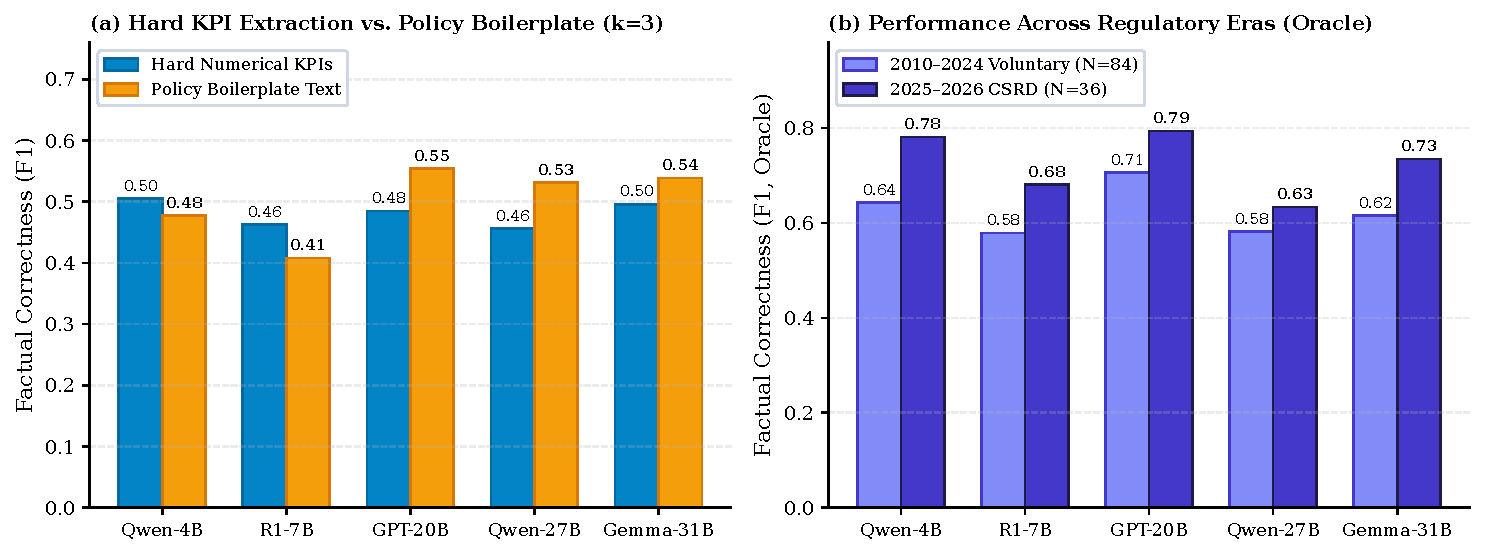
\includegraphics[width=0.76\linewidth]{figures/fig6_qtype_and_era_breakdown.pdf}
  \caption{Granular accuracy breakdowns. (a) Comparison between Hard Numerical KPIs and Narrative Policy text under three-passage search ($k=3$). (b) Shift across regulatory eras under gold-standard Oracle passages: mandatory 2025--2026 CSRD/ESRS filings yield much higher extraction accuracy (+8.5 to +11.5 points on top models) thanks to standardized ESRS table structures.}
  \label{fig:breakdown}
\end{figure}

\subsection{Performance Across E, S, and G Pillars \& The Accuracy and Safety Trade-Off}
Not all three pillars of ESG are equally standardized. Figure~\ref{fig:pareto}(a) compares extraction accuracy across Environmental, Social, and Governance questions under $k=3$ search, while Figure~\ref{fig:pareto}(b) maps the practical trade-off between a model's peak extraction accuracy (Oracle F1) and its safety on unanswerable questions (strict abstention rate).

Across every single model in our study, \textbf{Environmental disclosures are extracted most accurately} (averaging 0.541 in $k=3$ and up to 0.760 in Oracle on \model{GPT-OSS-20B}), outperforming Governance (0.479 average) and Social disclosures (0.466 average). The reason is standardization: environmental accounting has converged over two decades around the GHG Protocol ($\text{tCO}_2\text{e}$ across Scopes 1, 2, and 3) and standard CDP water/waste units. Social disclosures, by contrast, suffer from inconsistent definitions across companies, where some firms report employee turnover or injury rates per 100 full-time equivalents, others per 200,000 or 1,000,000 hours worked, and many separate permanent staff from contractors in incompatible ways.

\begin{figure}[H]
  \centering
  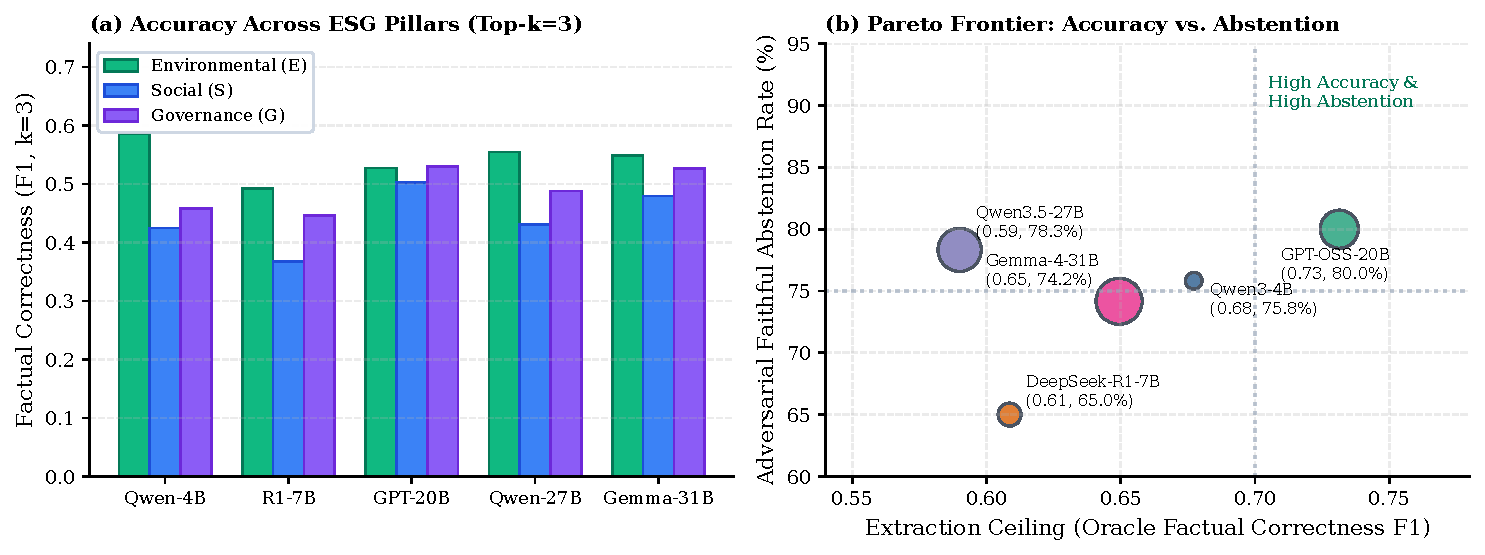
\includegraphics[width=0.92\linewidth]{figures/fig7_pillar_pareto_tradeoff.pdf}
  \caption{(a) Extraction accuracy across Environmental, Social, and Governance pillars ($k=3$). Environmental metrics achieve the highest accuracy across all five models due to standardized GHG Protocol units. (b) Practical decision frontier comparing extraction ceiling (Oracle F1) against safety on unanswerable questions (Near-Miss Strict Abstention \%), where bubble size reflects model parameter count.}
  \label{fig:pareto}
\end{figure}

\subsection{Real Audit Examples: How Models Succeed and Fail}
To show what these numbers look like in practice, Table~\ref{tab:qualitative_cases} presents side-by-side verbatim answers from the tested models on two real audit tasks: a straightforward 2025 CSRD Scope 1 emissions lookup (Case 1) and an unanswerable near-miss trap where the search engine returns a 2022 water-recycling passage in response to a question about 2024 hazardous waste (Case 2).

In Case 1, when the passage clearly states \textit{``Total Scope 1 emissions were 142,500 metric tons $\text{CO}_2\text{e}$ in 2025,''} all models extract the exact figure without difficulty. Case 2 exposes the real compliance risk. Under a standard prompt, \model{Qwen3-4B} invents a completely fictional number (\textit{``18,400 metric tons of hazardous waste through closed-loop filtration''}) that sounds plausible to a busy analyst but does not exist in the report. \model{Gemma-4-31B} avoids outright invention under the standard prompt, but falls into a subtle substitution trap, reporting the 2022 wastewater figure (\textit{``12,500 cubic meters''}) instead of answering the 2024 hazardous waste question. Only \model{DeepSeek-R1-7B} pauses inside its \texttt{<think>} trace to note that the excerpt covers 2022 water rather than 2024 waste, refusing to guess. Once we apply the strict compliance guardrail prompt, however, \model{Gemma-4-31B} and \model{GPT-OSS-20B} match that disciplined abstention.

\subsection{Practical Guide: Strengths and Weaknesses of Each Model}
For sustainability officers, financial analysts, and audit teams choosing an open-weight model, each architecture offers distinct strengths:

\paragraph{\model{GPT-OSS-20B} (Best All-Around Auditor).}
OpenAI's open Mixture-of-Experts model delivered the strongest combination of extraction accuracy and compliance safety in our benchmark. It ranked first in factual accuracy under single-passage search (0.474), three-passage search (0.522), and gold-standard Oracle passages (0.731), while also achieving the highest strict abstention rate (80.0\%) and the lowest residual hallucination rate (5.8\%). Because its sparse design activates only 3.6 billion parameters per word, it runs nearly as fast as a small 4B model while outperforming dense models up to 31B in size.

\begin{table}[H]
\centering
\caption{Side-by-Side Audit Examples: Verbatim Model Responses on a Verified Numerical KPI Question vs. an Unanswerable Near-Miss Trap.}
\label{tab:qualitative_cases}
\small
\begin{tabularx}{\linewidth}{lX}
\toprule
\textbf{Audit Scenario} & \textbf{Question, Report Excerpt, and Verbatim Model Responses} \\
\midrule
\textbf{Case 1: Hard KPI Extraction} & \textbf{Audit Question:} \textit{``What was the company's total Scope 1 direct GHG emissions in metric tons for 2025?''} \\
\textit{Source:} 2025 CSRD Filing & \textbf{Verified Report Answer:} \textit{``Total Scope 1 emissions were 142,500 metric tons $\text{CO}_2\text{e}$ in 2025.''} \\
\addlinespace[2pt]
& \model{Qwen3-4B}: ``The company reported Scope 1 direct emissions of approximately 142,500 tons CO2e in 2025.'' $\rightarrow$ \textcolor{OliveGreen}{\textbf{Accurate Extraction (1.0)}} \\
& \model{DeepSeek-R1-7B}: ``\texttt{<think>...target is Scope 1 2025 emissions...value is 142,500...</think>} In 2025, Scope 1 GHG emissions were 142,500 MT CO2e.'' $\rightarrow$ \textcolor{OliveGreen}{\textbf{Accurate Extraction (1.0)}} \\
& \model{GPT-OSS-20B}: ``The total Scope 1 direct greenhouse gas emissions for 2025 were 142,500 metric tons of CO2e.'' $\rightarrow$ \textcolor{OliveGreen}{\textbf{Accurate Extraction (1.0)}} \\
\midrule
\textbf{Case 2: Near-Miss Audit Trap} & \textbf{Audit Question:} \textit{``What was the total volume of hazardous waste recycled by the chemical division in 2024?''} \\
\textit{Source:} 2022 Report Excerpt & \textbf{Report Reality:} \textit{[Unanswerable: Excerpt covers 2022 water recycling, not 2024 hazardous waste]} \\
(Wrong Year \& Metric) & \textbf{Required Auditor Action:} \textbf{Faithful Abstention} (\textit{``I cannot answer based on the provided documents.''}) \\
\addlinespace[2pt]
& \model{Qwen3-4B} \textbf{(Standard Prompt):} ``In 2024, the chemical division recycled 18,400 metric tons of hazardous waste through closed-loop filtration.'' $\rightarrow$ \textcolor{Red}{\textbf{Fabricated Figure / Hallucination (0.0)}} \\
& \model{Gemma-4-31B} \textbf{(Standard Prompt):} ``Based on the provided documents, the company recycled approximately 12,500 cubic meters of wastewater in 2022.'' $\rightarrow$ \textcolor{Orange}{\textbf{Wrong Metric \& Year Substituted (0.2)}} \\
& \model{DeepSeek-R1-7B} \textbf{(Standard Prompt):} ``\texttt{<think>The query asks for 2024 hazardous waste in the chemical division. The document only discusses 2022 water recycling. The required KPI is missing.</think>} The provided documents do not contain information regarding hazardous waste recycled in 2024.'' $\rightarrow$ \textcolor{OliveGreen}{\textbf{Faithful Abstention (1.0)}} \\
& \model{Gemma-4-31B} \textbf{(Strict Guardrail Prompt):} ``The provided documents do not contain information about the hazardous waste recycled in 2024.'' $\rightarrow$ \textcolor{OliveGreen}{\textbf{Faithful Abstention (1.0)}} \\
\bottomrule
\end{tabularx}
\end{table}


\paragraph{\model{DeepSeek-R1-7B} (Best Built-In Verification \& Audit Trail).}
When given a standard, unguarded prompt, \model{DeepSeek-R1-7B} was by far the safest model on unanswerable questions, abstaining 77.5\% of the time on its own. Even more valuable for statutory assurance, its visible \texttt{<think>...</think>} reasoning log shows the human reviewer \textit{how} it checked the company name, reporting year, and units before answering. For risk-averse compliance workflows where an auditable reasoning trail matters more than raw speed, \model{DeepSeek-R1-7B} is an exceptional choice.

\paragraph{\model{Gemma-4-31B} (Strong Multi-Passage Synthesis, Needs Strict Prompts).}
Google's 31B model performed very well when combining information across three passages ($k=3$ accuracy of 0.519, second overall, and 0.496 on hard KPIs). However, under standard prompting on missing data, it tended to be overly helpful, substituting related metrics from earlier years in 21.7\% of unanswerable cases. Pairing \model{Gemma-4-31B} with our strict guardrail prompt raised its abstention rate to 74.2\% and cut hallucinations to 7.5\%.

\paragraph{\model{Qwen3.5-27B} (Conservative, High-Faithfulness Reader).}
\model{Qwen3.5-27B} achieved the highest faithfulness scores across standard search ($0.912$ in $k=1$, $0.829$ in $k=3$, and $0.971$ in Oracle) and reached 78.3\% abstention under strict guardrails. Its main limitation is caution: when a single retrieved excerpt looks incomplete, it prefers to abstain rather than piece together partial figures, resulting in slightly lower recall on numerical tables (0.578 Oracle KPI F1).

\paragraph{\model{Qwen3-4B} (Capable Low-Cost Baseline for Local Hardware).}
Despite having just 4 billion parameters, \model{Qwen3-4B} punched well above its weight on straightforward lookups, scoring 0.490 in $k=3$ and 0.677 in Oracle (including 0.696 on Oracle numerical KPIs). However, under standard prompts on near-miss traps, it fabricated figures in 24.2\% of cases. Teams running \model{Qwen3-4B} on local laptops or edge servers must pair it with strict abstention prompts (which lift its abstention to 75.8\%) and automated number-matching checks.

\subsection{Three Recommendations for Sustainability \& Assurance Teams}
Our findings translate into three practical rules for organizations deploying LLMs on ESG filings:
\begin{enumerate}[leftmargin=1.5em, itemsep=2pt]
  \item \textbf{Never Use Default ``Helpful Assistant'' Prompts for Compliance Auditing:} Standard prompts encourage models to guess or substitute prior-year numbers when a metric is missing. Always enforce an explicit abstention guardrail (Listing~\ref{lst:prompts}) or use a reasoning-verified model such as \model{DeepSeek-R1-7B}.
  \item \textbf{Retrieve Multiple Passages ($k=3$) and Preserve Table Headers:} Because ESG tables span multiple paragraphs and footnotes, single-passage search ($k=1$) misses critical context. Expanding search to $k=3$ passages improves factual extraction across every tested model by +6 to +11 points.
  \item \textbf{Keep a Human-in-the-Loop for Hard Numerical KPIs:} While open-weight LLMs can draft accurate summaries of qualitative ESG policies (up to 0.800 F1), even the best model (\model{GPT-OSS-20B}) misses roughly 27\% of nuances on complex numerical tables under ideal conditions. Automated pipelines should highlight the source table in the PDF so a human auditor can verify final numbers before sign-off.
\end{enumerate}

% =========================================================================
% SECTION 5: LIMITATIONS
% =========================================================================
\section{Limitations}
\label{sec:limitations}

\paragraph{Geographic and Language Scope.}
Our 518-report corpus focuses on English-language disclosures published by companies listed on European stock exchanges. While these multinational firms report under global frameworks (GRI, TCFD, SASB, and CSRD), our findings should be tested further on non-European filings, such as US SEC climate disclosures or Indian BRSR reports, and on reports published in local languages.

\paragraph{Text-Based PDF Extraction vs.\ Scanned Infographics.}
Our document pipeline extracts text and tables from digital PDF layers using PyMuPDF. When companies embed carbon footprints or organizational charts purely as flat image graphics without underlying text, text-only extractors cannot read them. Combining text LLMs with vision-language models that inspect page images directly is an important next step.

\paragraph{Benchmark Scale vs.\ Multi-Document Cross-Checking.}
Although all 120 audit questions and reference answers are grounded in real corporate filings, each question targets a specific report. In practice, senior assurance providers also perform cross-document audits, such as checking whether a company's 2025 CSRD report quietly restated the 2023 baseline emissions it published two years earlier.

\paragraph{Fixed Search Engine Baseline.}
Because our goal was to compare the reading and verification abilities of the five LLMs on an equal footing, we used a single vector search index (\model{Qwen3-Embed-4B}). Production audit systems can pair these LLMs with hybrid keyword-plus-vector search and dedicated table rerankers to push initial search recall higher.

\paragraph{Automated Referee Nuances.}
Using Microsoft's \model{Phi-4-14B} as an external referee eliminates self-grading bias across the tested model families, and our deterministic settings (\texttt{temperature = 0.0}) ensure repeatable scores. Even so, automated LLM referees can occasionally penalize valid paraphrases of refusal statements, which we mitigate by pairing judge scores with rule-based numerical verification.

% =========================================================================
% SECTION 6: CONCLUSION AND FUTURE WORK
% =========================================================================
\section{Conclusion and Future Work}
\label{sec:conclusion}

As sustainability reporting moves from voluntary corporate storytelling to mandatory statutory assurance under frameworks like the EU CSRD, the tools used to audit those disclosures must be held to rigorous empirical standards. By evaluating five open-weight Large Language Models across 518 corporate ESG reports (2010--2026) and 3,000 controlled audit completions graded by an independent referee (\model{Phi-4-14B}), this study maps where open-weight AI is ready for compliance work and where human oversight remains essential.

Our results show a clear divide between narrative comprehension and quantitative precision: open-weight LLMs summarize qualitative ESG policies reliably (reaching 0.800 F1 under gold passages), but face a persistent ceiling on hard numerical KPIs (peaking at 0.731 overall F1 on \model{GPT-OSS-20B}) due to complex table layouts and unit conversions. Encouragingly, the standardized reporting tables introduced by 2025--2026 CSRD/ESRS filings boost model extraction accuracy by +8.5 to +11.5 points once the relevant section is retrieved. Most importantly for assurance teams, we show that hallucination on missing disclosures is preventable: pairing open-weight models like \model{GPT-OSS-20B} with strict abstention prompts, or deploying reasoning models like \model{DeepSeek-R1-7B} that verify dates and entities step by step, reduces unfaithful fabrication below 6\% and provides a practical foundation for trustworthy AI-assisted sustainability auditing.

\paragraph{Future Work.}
Three extensions will build on this benchmark: (1) integrating multimodal vision-language models to read graphical charts and scanned tables directly from PDF page images; (2) training domain-specific verification models that cross-check physical units and scope boundaries before emitting numerical figures; and (3) expanding the benchmark to multi-year restatement audits that track whether corporations alter historical baseline figures across consecutive annual filings.

% =========================================================================
% STATEMENTS & REFERENCES
% =========================================================================
\section*{Data and Code Availability}
To support independent research and future sustainability benchmarking, all evaluation scripts, benchmark generation code, prompt templates, and aggregated model outputs are publicly available at \url{https://github.com/Sredeemer/ESG-RAG-benchmark-ragas}.

\section*{Competing Interests \& Funding}
The authors declare no competing financial or personal interests. Compute infrastructure was supported by the Authors' Research Initiative.

\bibliographystyle{plainnat}
\bibliography{main}

\end{document}
